A Tabela \ref{tab:tempos_selection} apresenta os tempos de execução, em segundos, obtidos para o Selection Sort nos seis tamanhos de instância exigidos pelo trabalho, para cada um dos três tipos de entrada testados.

\begin{table}[htbp]
    \centering
    \begin{tabular}{|l|r|r|r|r|r|r|}
        \hline
         & 10 & 100 & 1.000 & 10.000 & 100.000 & 1.000.000 \\
        \hline
        Crescente & 0,000001 & 0,000008 & 0,001218 & 0,125560 & 12,468661 & 323,090207 \\
        \hline
        Decrescente & 0,000001 & 0,000010 & 0,001194 & 0,122701 & 12,588413 & 306,210246 \\
        \hline
        Random & 0,000001 & 0,000013 & 0,001230 & 0,116897 & 12,419415 & 321,875258 \\
        \hline
    \end{tabular}
    \caption{Tempo de execução (em segundos) do Selection Sort por tamanho e tipo de instância}
    \label{tab:tempos_selection}
\end{table}

O Gráfico \ref{fig:grafico_selection} apresenta esses mesmos dados em escala linear. Diferentemente do Insertion Sort, aqui as três curvas ficam praticamente sobrepostas em todos os tamanhos, o que já era esperado pela análise de complexidade: o número de comparações do Selection Sort não depende do tipo de entrada.

\begin{figure}[htbp]
    \centering
    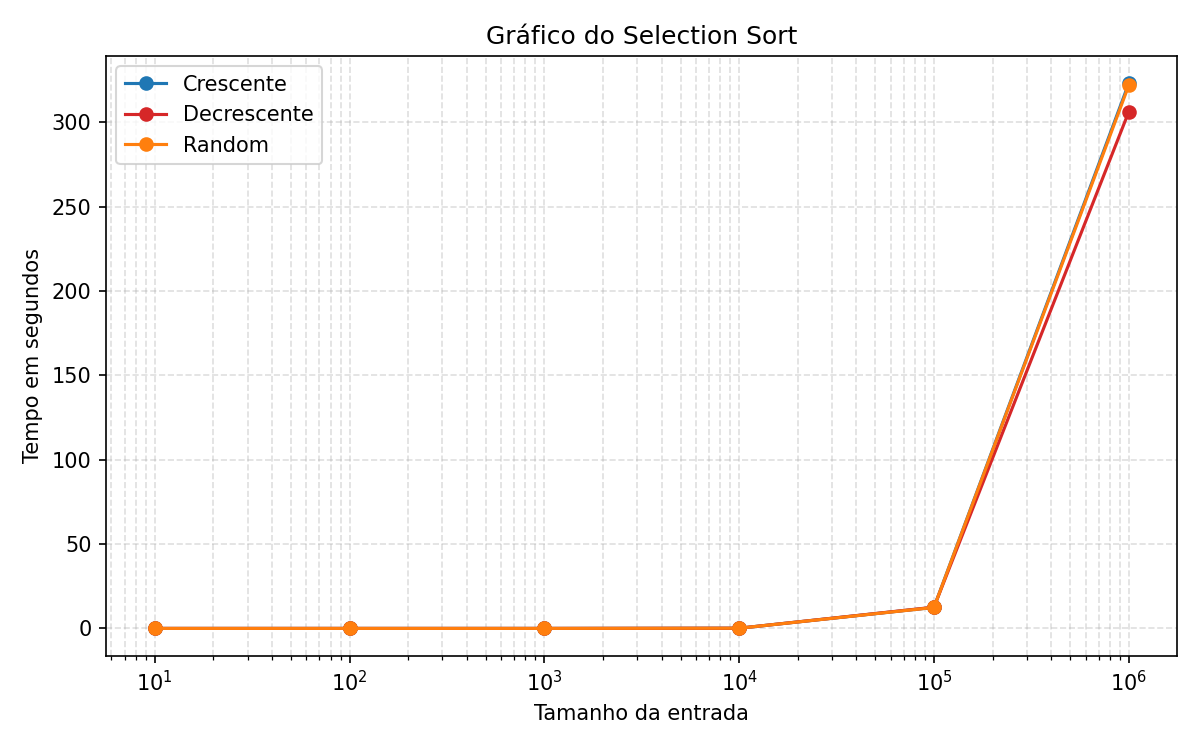
\includegraphics[width=14cm]{Imagens/Selection Sort/grafico.png}
    \caption{Gráfico de tempo por tamanho do algoritmo Selection Sort (escala linear)}
    \label{fig:grafico_selection}
\end{figure}

Como as três curvas são muito próximas, o Gráfico \ref{fig:grafico_selection_log} em escala logarítmica ajuda a confirmar que, mesmo em pequena escala, os tempos de Crescente, Decrescente e Random seguem lado a lado durante todo o intervalo de tamanhos testado -- a assinatura característica de um algoritmo cujo número de comparações independe da ordem dos dados de entrada, conforme discutido na análise de complexidade deste capítulo.

\begin{figure}[htbp]
    \centering
    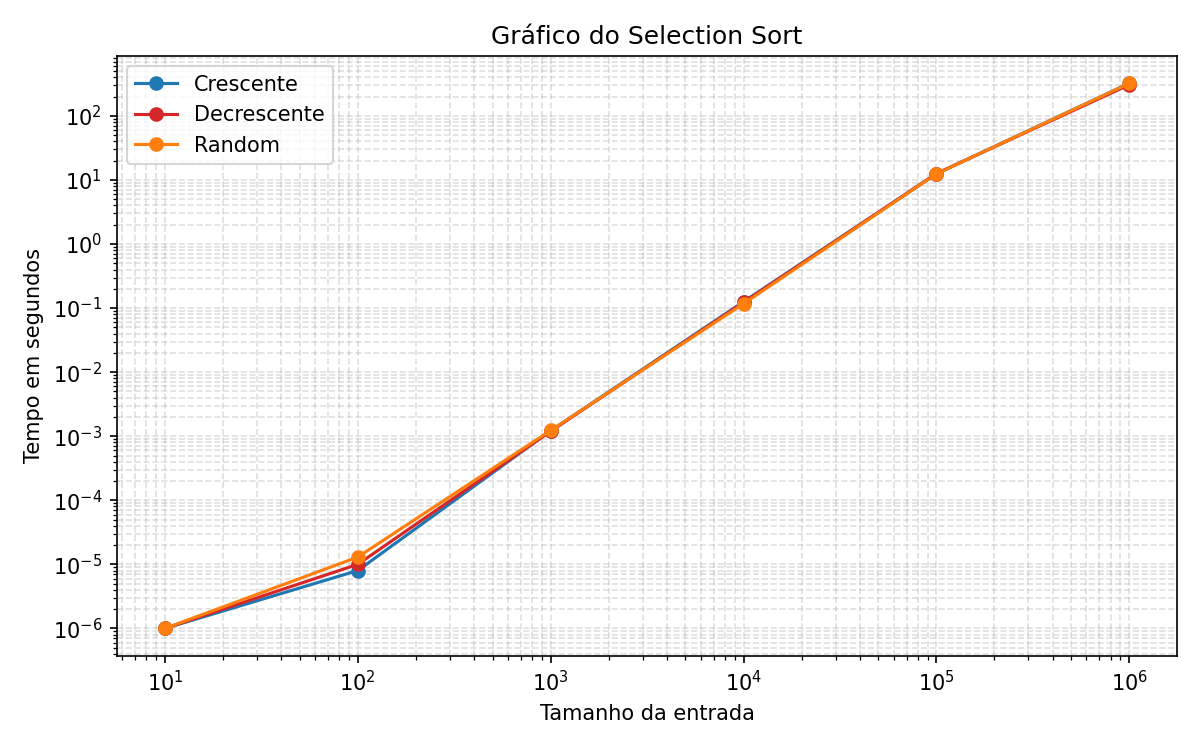
\includegraphics[width=14cm]{Imagens/Selection Sort/grafico_log.png}
    \caption{Gráfico de tempo por tamanho do algoritmo Selection Sort (escala logarítmica)}
    \label{fig:grafico_selection_log}
\end{figure}
